\section{Discussion}
\note{
    \begin{itemize}
        \item 4 threats we did not account for
    \end{itemize}
}

\metroset{block=transparent}

\subsection{Unmitigated Threats}

\begin{frame}{Exploring Unmitigated Threats}
    \begin{columns}[T,onlytextwidth]
        \column{0.47\textwidth}
        \pause

        \begin{block}{Cryptography Exploit}
            \begin{itemize}

                \item Beacon not dependent on any algorithm
            \end{itemize}
        \end{block}
        \pause
        \begin{block}{Eclipse Attacks}
            \begin{itemize}
                \item Have multiple connections to outside world
            \end{itemize}
        \end{block}

        \column{0.47\textwidth}
        \pause
        \begin{block}{Operator Shutdown}
            \begin{itemize}
                \item Only disrupts use cases
            \end{itemize}
        \end{block}

        \pause
        \begin{block}{Input Flooding}
          \begin{itemize}
              \item Rate limiting
              \item Proof-of-Work puzzle
          \end{itemize}
        \end{block}

    \end{columns}
\note{
    \begin{multicols}{2}
        \begin{itemize}
            \item Cryptography Exploits
            \begin{itemize}
                \item (cannot anticipate these)
                \item We can mitigate if and when exploit is found
            \end{itemize}
            
            \item Eclipse Attacks
            \begin{itemize}
                \item Not much we can do, besides
                \item Perhaps even other ways besides internet
                \begin{itemize}
                    \item Wireless option: SMS
                \end{itemize}
            \end{itemize}

            \item Operator Shutdown
            \begin{itemize}
                \item Downside of having single authority
                \item The attack is about: shutting down beacon \textrightarrow{} not even accept input
                \begin{itemize}
                    \item Users will not have stake in it
                    \item Operator will not gain any benefit
                    \item ... only disrupting uses cases relying on beacon
                \end{itemize}
            \end{itemize}

            \item Input Flooding
            \begin{itemize}
                \item Real risk, but not just for beacons
                \item Many existing ways to migitage
                \item Rate limiting to acceptable level
                \item Investigate proof-of-work
                \begin{itemize}
                    \item Solve computationally hard puzzle
                \end{itemize}
            \end{itemize}
        \end{itemize}
    \end{multicols}
}\end{frame}


\subsection{Alternative Delay Functions}

\begin{frame}{Alternative Delay Functions}
    \centering
    A dedicated ASIC to compute \emph{sloth} may be faster.
    \\
    \vspace{1cm}
    Adversary with ASIC must also be able to execute an attack.
\end{frame}
\note{
    \begin{itemize}
        \item Choice of sloth may be re-considered
        \item Presumably, dedicated hardware...
        \item How much faster? Good question
        \begin{itemize}
            \item Few orders of magnitude might pose a problem
        \end{itemize}
        \item Posessing an ASIC not enough \textrightarrow{} also launch attack
        \item Since the OP can buy ASIC, we must deter usage of them
    \end{itemize}
}

\begin{frame}{Alternative Delay Functions}
    \centering
    \textbf{Two solutions:}

    \vspace{.5cm}
    
    \begin{columns}[T, onlytextwidth]
        \column{0.47\textwidth}
        \begin{block}{Use Memory-Hard Delay Function}
            \begin{itemize}
                \item ASICs have limited memory
                \item Memory is slow in large quantities
            \end{itemize}
        \end{block}

        \column{0.47\textwidth}
        \begin{block}{Change Delay Function}
            \begin{itemize}
                \item ASIC: expensive and hard-wired
                \item Beacon: Changing or permutating delay function is free
            \end{itemize}
        \end{block}
    \end{columns}
\end{frame}
\note{
    \begin{itemize}
        \item ASIC can be counteracted by either
        \begin{itemize}
            \item requiring a lot of memory
            \item changing or permutating delay faster
        \end{itemize}
        \item ASICs have limited memory
        \begin{itemize}
            \item if much memory required \textrightarrow{} cost-prohibitive to have fast memory
            \item 1-2 gb required \textrightarrow{} must be normal computer ram
            \item slow compared to rest of ASIC \textrightarrow{} bottleneck (CPU-comparable levels)
        \end{itemize}
        \item Change / Permutate Delay Function
        \begin{itemize}
            \item ASIC is designed for 1 purpose \textrightarrow{} One-trick pony
            \begin{itemize}
                \item Does 1 thing, hard-wired
            \end{itemize}
            \item Changing / Permutating \textrightarrow{} redesign of ASIC (expensive)
            \item No dependency on delay function, trivially change it.
        \end{itemize}
    \end{itemize}
}

\begin{frame}{Rational Trust}
    \note{
    \begin{multicols}{2}
        \begin{itemize}
            \item In paper: user needs to trust input (by himself / other user, doesn't matter)
            \begin{itemize}
                \item We have thought more about this, and specify it more precisely:
                \item SLIDE (at least two non-colluding disjoint sets of input)
            \end{itemize}
            \item So even if one half is colluding, and other, too
            \begin{itemize}
                \item Output is secure
                \item Two halves are \textbf{counteracting} eachother
            \end{itemize}
            \item A set may just consist of one input
            \begin{itemize}
                \item and to make sure of two non-colluding sets, SLIDE this should be your input
                \item Even if all other inputs in this set over here are colluding, the output is secure
            \end{itemize}
            \item If you relax your requirements as a user
            \begin{itemize}
                \item if not contributing, you can still trust in some circumstances
                \item You know two users contributed. Not trust them, but you believe they did not collude
            \end{itemize}
        \end{itemize}
    \end{multicols}
    }
    \pause
    \centering
    \enquote{The beacon is secure if there are (at least)\\\textbf{two non-colluding disjoint sets of input}}
    
    \pause
    \vspace{.3cm}
    \begin{tikzpicture}
        \draw[ultra thick] (0,0) ellipse (1 and 2)
            (4,0) ellipse (1 and 2);
        % \clip (0,0) ellipse (1 and 2) (4,0) ellipse (1 and 2);
        \only<3>{
            \fill (0.5, 0.9) circle(1.5pt);
            \fill (-0.3, 1.3) circle(1.5pt);
            \fill (-0.2, -1.4) circle(1.5pt);
            \fill (-0.7, 0.1) circle(1.5pt);
        }
        \only<1-5>{
            \fill (0.3, -0.4) circle(1.5pt);
        }
        \only<5>{
            \coordinate (end) at (0.3, -0.4);
            \coordinate (start) at (1.5, -1);
            \draw[-latex, shorten <=3pt, thick, draw=red] (start) -- (end);
        }

        \fill (3.7, 1.4) circle(1.5pt);
        \fill (4.2, -1.6) circle(1.5pt);
        \fill (3.7, -0.5) circle(1.5pt);
        \fill (4.7, 0.1) circle(1.5pt);
    \end{tikzpicture}

\end{frame}


\subsection{Practicalities}

\begin{frame}{Practicalities: Stopping in a Fair Way}
    \note{
        \begin{itemize}
            \item A necessity that turns up: Extend input coll. time to more than beacon's ict
            \item It turns out:
            \begin{itemize}
                \item fresh randomness with high frequency
                \item in some cases: a long input collection time
                \item (all involved users need to see one common commit)
            \end{itemize}
            \item Pattern we quickly discovered 
            \item Solution: perform ceremony that combines several outputs
            \begin{itemize}
                \item with last output being determined by a "stop"-message.
            \end{itemize}
            \item This way, security goals of beacon are extended to use cases
            \begin{itemize}
                \item Entity controlling when to stop, cannot know when it is most beneficial.
                \item Can only see the result afterwards
            \end{itemize}
        \end{itemize}
    }
    \textbf{Desirable beacon properties:}
    \begin{itemize}
        \item High output frequency
        \item Long input collection time
    \end{itemize}

    \vspace{.7cm}
    \centering
    \pause
    Solution: Ceremonies on top of beacon

    \vspace{.3em}
    \pause
    Standardize this common pattern

\end{frame}

\begin{frame}{Practicalities: Extending Trust into the Reality}
    \note{
        \begin{itemize}
            \item Last point I want to talk about is how to extend trust real life
            \begin{itemize}
                \item A problem blockchains currently face, don't have a good solution for
            \end{itemize}
            \item Essentially, (how ensure lottery pays money)
            \begin{itemize}
                \item today, trust, reputation is important
            \end{itemize}
            \item In the future, if cryptocurrencies are widespread
            \begin{itemize}
                \item Smart contracts lock-in funds in lottery, and automatically pays out prize to winner.
                \item Beacon is a primitive. Users in lottery also needs input to beacon.
            \end{itemize}
            \item Brings up questions:
            \begin{itemize}
                \item How can output be transfered to smart contract securely?
            \end{itemize}
            \item Today, users don't want prize in cryptocurrency. And so, trust is still needed for use cases that bridge to the real world.
        \end{itemize}
    }
    How can we ensure that the lottery pays the money?
    \pause
    \begin{itemize}
        \item Trust them
        \pause
        \item Cryptocurrencies and smart contracts
    \end{itemize}
\end{frame}

\begin{frame}{Summary}
    Succinct beacon design and implementation
    \begin{itemize}
        \item Enumerate threats
        \item Describe usage of beacon in context
        % \item Of more technical nature:
    \end{itemize}
    \begin{itemize}
        \item Parallelize pipeline
        \item Early release of inputs (CCO)
        \item Multiple input/output channels
        \item Usage of Merkle trees
    \end{itemize}
\end{frame}
\note{
    \begin{itemize}
        \item All in all:
        \begin{itemize}
            \item explored, designed, implemented RB with succinct operation.
        \end{itemize} 
        \item More concretely, we fill a gap in current literature with the following points:
        \begin{itemize}
            \item Enumerate threats: previous papers don't do this up-front and more casually mentions threats as an after-thought to their design.
            \item Describe usage of beacon in real world context: Other papers just mention, and not how to properly apply
            \item \textbf{Of more technical nature:}
            \begin{itemize}
            \item Explicitly consider how to parallelize (not considered before)
            \item We re-think flow of transparent authorities, inputs released early (mitigate output withholding attacks).
            \item Allow multiple input/output channels (first ones to explore more than a sidenote)
            \item Finally, we use Merkle trees for structuring inputs (decreases proof size for regular users, as far as we know: only beacon that does this)
            \end{itemize}
        \end{itemize}
    \end{itemize}
}
